\section{Applications to FASER}
\label{sec:faser-app}
\label{sec:rates}

The comparisons presented so far are carried out at fixed $E_\ell$ values.
%
Here we use the same pipeline together with the LHC electron- and muon-neutrino fluxes~\cite{FASER:2024ykc} to provide predictions for representative observables at FASER.
%
We consider three specific applications: comparison of generator predictions with the latest FASER data from the emulsion and electronic sub-detectors, a study of the PDF dependence in the predictions for the dimuon signal at FASER's electronic detector, and predictions for charged-hadron production in SIDIS at FASER$\nu$. 
%
The expected number of events for a fiducial selection is 
\be
  N \, = \, \int dE_\nu \; \Phi(E_\nu) \, \sigma_{\rm fid}(E_\nu) \, T \, ,
  \label{eq:rate}
\ee
with $\Phi$ the neutrino flux through the detector for a given integrated luminosity~\cite{Kling:2021gos}, $T$ the column density of the tungsten target, and $\sigma_{\rm fid}$ the fiducial cross-section per nucleon, evaluated as explained in Sect.~\ref{sec:settings} from separate proton and neutron samples.
%
The cross-section in Eq.~(\ref{eq:rate}) is required as a continuous function of $E_\nu$, and
here we build a common fine energy ladder from $10$~GeV to several TeV from the \yadism NLO ZM prediction and then rescale it, for each generator, by its ratio to \yadism interpolated in $\log E_\nu$ between the energies at which that generator has been run.
%
In the following, the FASER Run 3 flux model for $\Phi(E_\nu)$ in Eq.~(\ref{eq:rate}) is taken to be the same as in~\cite{FASER:2024ykc}, namely {\sc\small EPOS-LHC}~\cite{Pierog:2013ria} for light-hadron production and POWHEG-BOX heavy-quark production matched to \pythia~\cite{Buonocore:2023kna} for charm-hadron production, and no flux uncertainties are considered. 

\paragraph{Comparison with FASER data.}
%
The most recent FASER$\nu$ measurement~\cite{FASERnu:2026conf} reports $33$ muon-neutrino and $7$ electron-neutrino CC candidates collected with an integrated luminosity of $\mathcal{L}=9.5$~fb$^{-1}$.
%
Fig.~\ref{fig:faser-emulsion} compares four measured differential distributions ($N_{\tr}$, $\tan \theta_{\ell'}$, $p_{\ell'}$, $\Delta \phi$) for $\nu_e+\bar{\nu}_e$  and $\nu_\mu+\bar{\nu}_\mu$ from~\cite{FASERnu:2026conf} with the corresponding predictions from \powhegtwo, \sherpa, and \herwig as well as from \genie with the default tune (GRV98LO).
%
For each generator, distributions are normalised to the observed event yields to account for the experimental selection and acceptance efficiencies. 

%%%%%%%%%%%%%%%%%%%%%%%%%
\begin{figure}[!tbp]
  \centering
  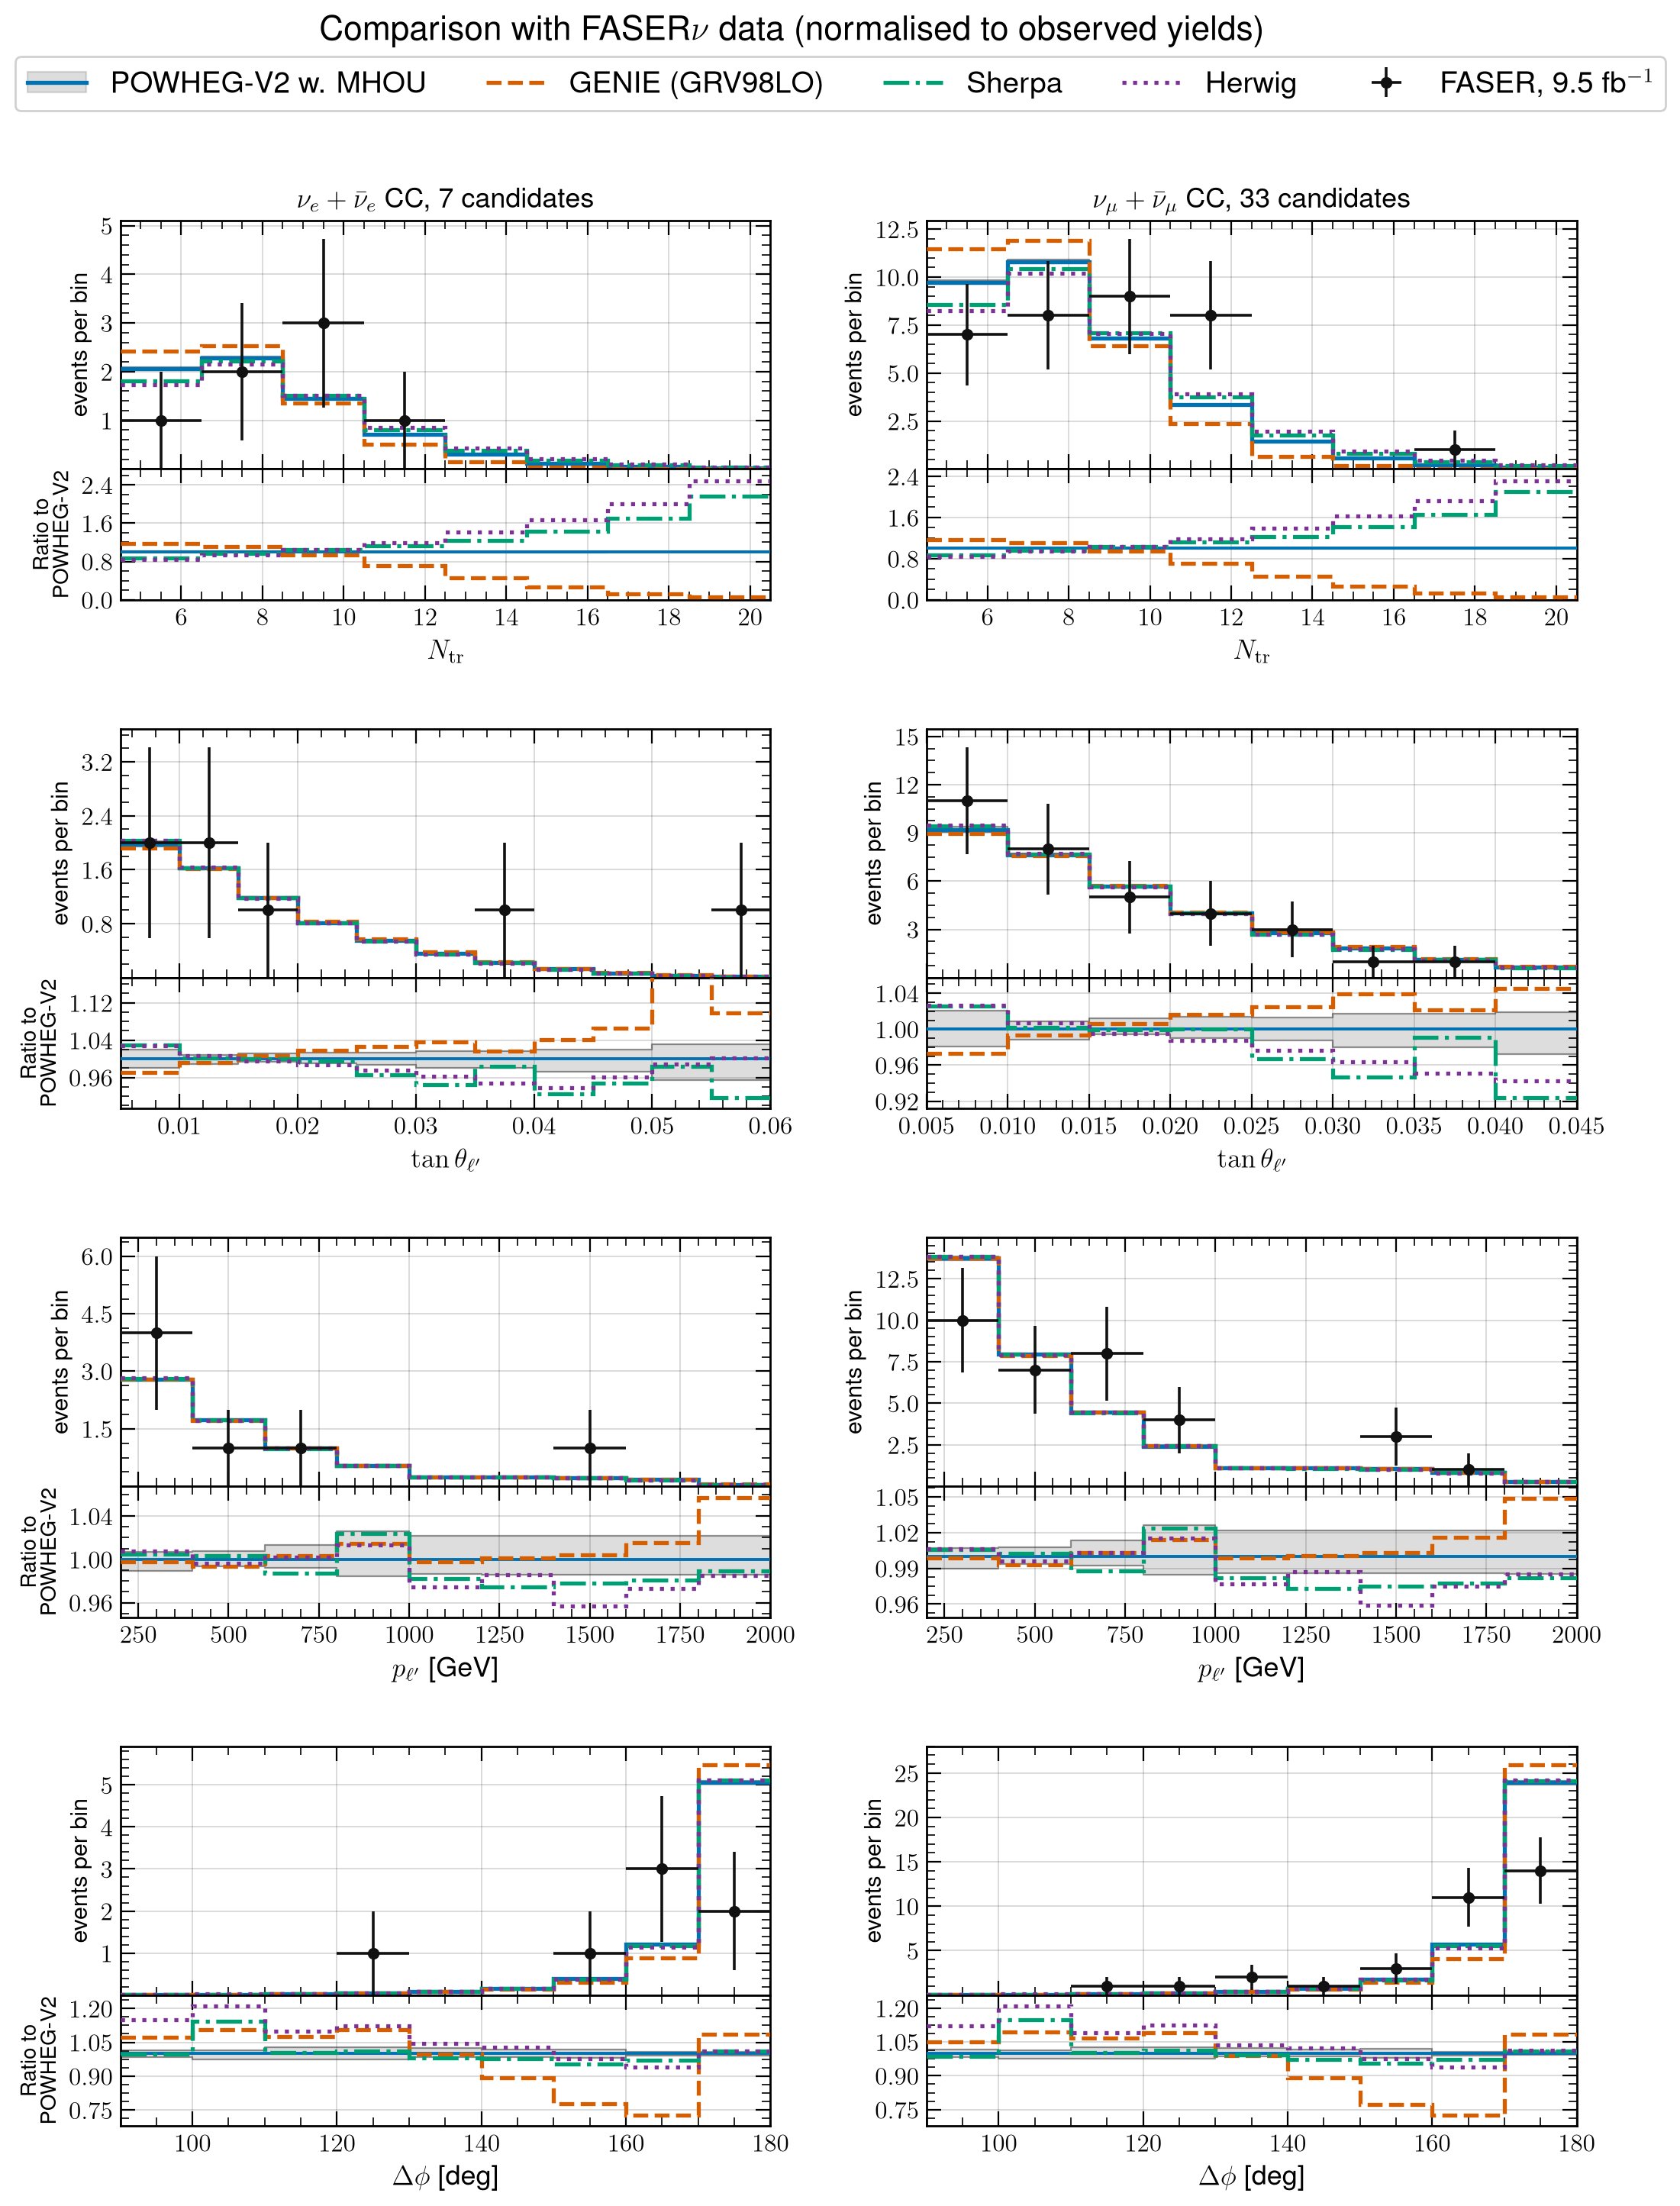
\includegraphics[width=0.95\textwidth]{figures/pp_faser_emulsion.png}
  \caption{Differential distributions for $\nu_e+\bar{\nu}_e$ (left panels) and $\nu_\mu+\bar{\nu}_\mu$ (right panels) charged-current DIS candidate events at FASER$\nu$ for $\mathcal{L}=9.5$ fb$^{-1}$~\cite{FASERnu:2026conf}.
  %
  From top to bottom, we show $N_{\tr}$, $\tan \theta_{\ell'}$, $p_{\ell'}$, and $\Delta \phi$ (defined as the azimuthal separation between the lepton and the summed remaining tracks).
   %
   We display the corresponding predictions from \powhegtwo, \sherpa, and \herwig with the benchmark settings as well as from \genie (GRV98LO). 
  %
  For each generator, distributions are normalised to the observed event yields.
  %
  The bottom panels show the ratio of each generator to the \powhegtwo predictions. }
  \label{fig:faser-emulsion}
\end{figure}
%%%%%%%%%%%%%%%%%%%%%%%%%%

The four predictions differ where the modelling of the  hadronic final state becomes relevant.
%
The outgoing lepton momentum and the scattering angle follow the agreement at the level of inclusive distributions found in Sect.~\ref{sec:inclusive}.
%
In particular, for $p_{\ell'}$ the four predictions agree to within $6\%$ in every bin.
%
On the track multiplicity distribution, \genie prefers lower values of $N_{\tr}$ as compared to \powhegtwo, \sherpa, and \herwig,  the same ordering found at fixed neutrino energy in Fig.~\ref{fig:hadron-level}.
%
For the azimuthal separation $\Delta\phi$, \genie lies around $7\%$ above \powhegtwo well below the back-to-back peak and a third below it just short of the peak, differences which are much larger than the estimated MHOUs.
%
For the bulk of the $\Delta\phi$ distribution, \powhegtwo, \sherpa, and \herwig display good agreement. 
%
While the limited statistics in the FASER$\nu$ measurement are not sufficient to arbitrate these differences, future data will constrain the modelling of the hadronic final state for this process, improving {\it e.g.} vertex selection. 

In addition to the neutrino emulsion data, FASER has also measured the $\nu_\mu$ and $\bar{\nu}_\mu$ CC interaction rate and fluxes with its electronic detector~\cite{FASER:2024ref,FASER:2026enu2d}, in bins of $-L/E_\nu$, where $L$ is the lepton number, using the spectrometer selection described in Sect.~\ref{sec:faser-selections}.
%
The latter measurement is also presented double-differentially in $E_\nu$ and in the neutrino rapidity, following an earlier measurement of the muon-neutrino flux as a function of rapidity~\cite{FASER:2025nurap}; here we compare only with its energy dependence, since the flux rapidity does not affect DIS modelling.
%
Fig.~\ref{fig:faser-electronic} displays the predictions from \powhegtwo, \sherpa, \herwig, and \genie for the flux-weighted cross-section for CC DIS for the kinematics of~\cite{FASER:2026enu2d}.
%
Since \powhegtwo, \sherpa, and \herwig predictions are generated for $Q^2>4$~GeV$^2$, while the FASER measurement corresponds to the total cross-section without a $Q^2$ cut, we extend these predictions with the $Q^2<4$~GeV$^2$ contribution estimated by \genie, which amounts to between $1\%$ and $23\%$ ($37\%$) of the $\nu_\mu$ ($\bar\nu_\mu$) cross-section from the highest to the lowest neutrino energies.
%
Then the right panel of Fig.~\ref{fig:faser-electronic} shows the corresponding predictions for the number of muon-neutrino CC interactions expected in the fiducial volume at $\mathcal{L}=186$~fb$^{-1}$ compared to the unfolded FASER data~\cite{FASER:2026enu2d}. 

%%%%%%%%%%%%%%%%%%%%%%%%%%%%%%%%%%%%%
\begin{figure}[!tbp]
  \centering
  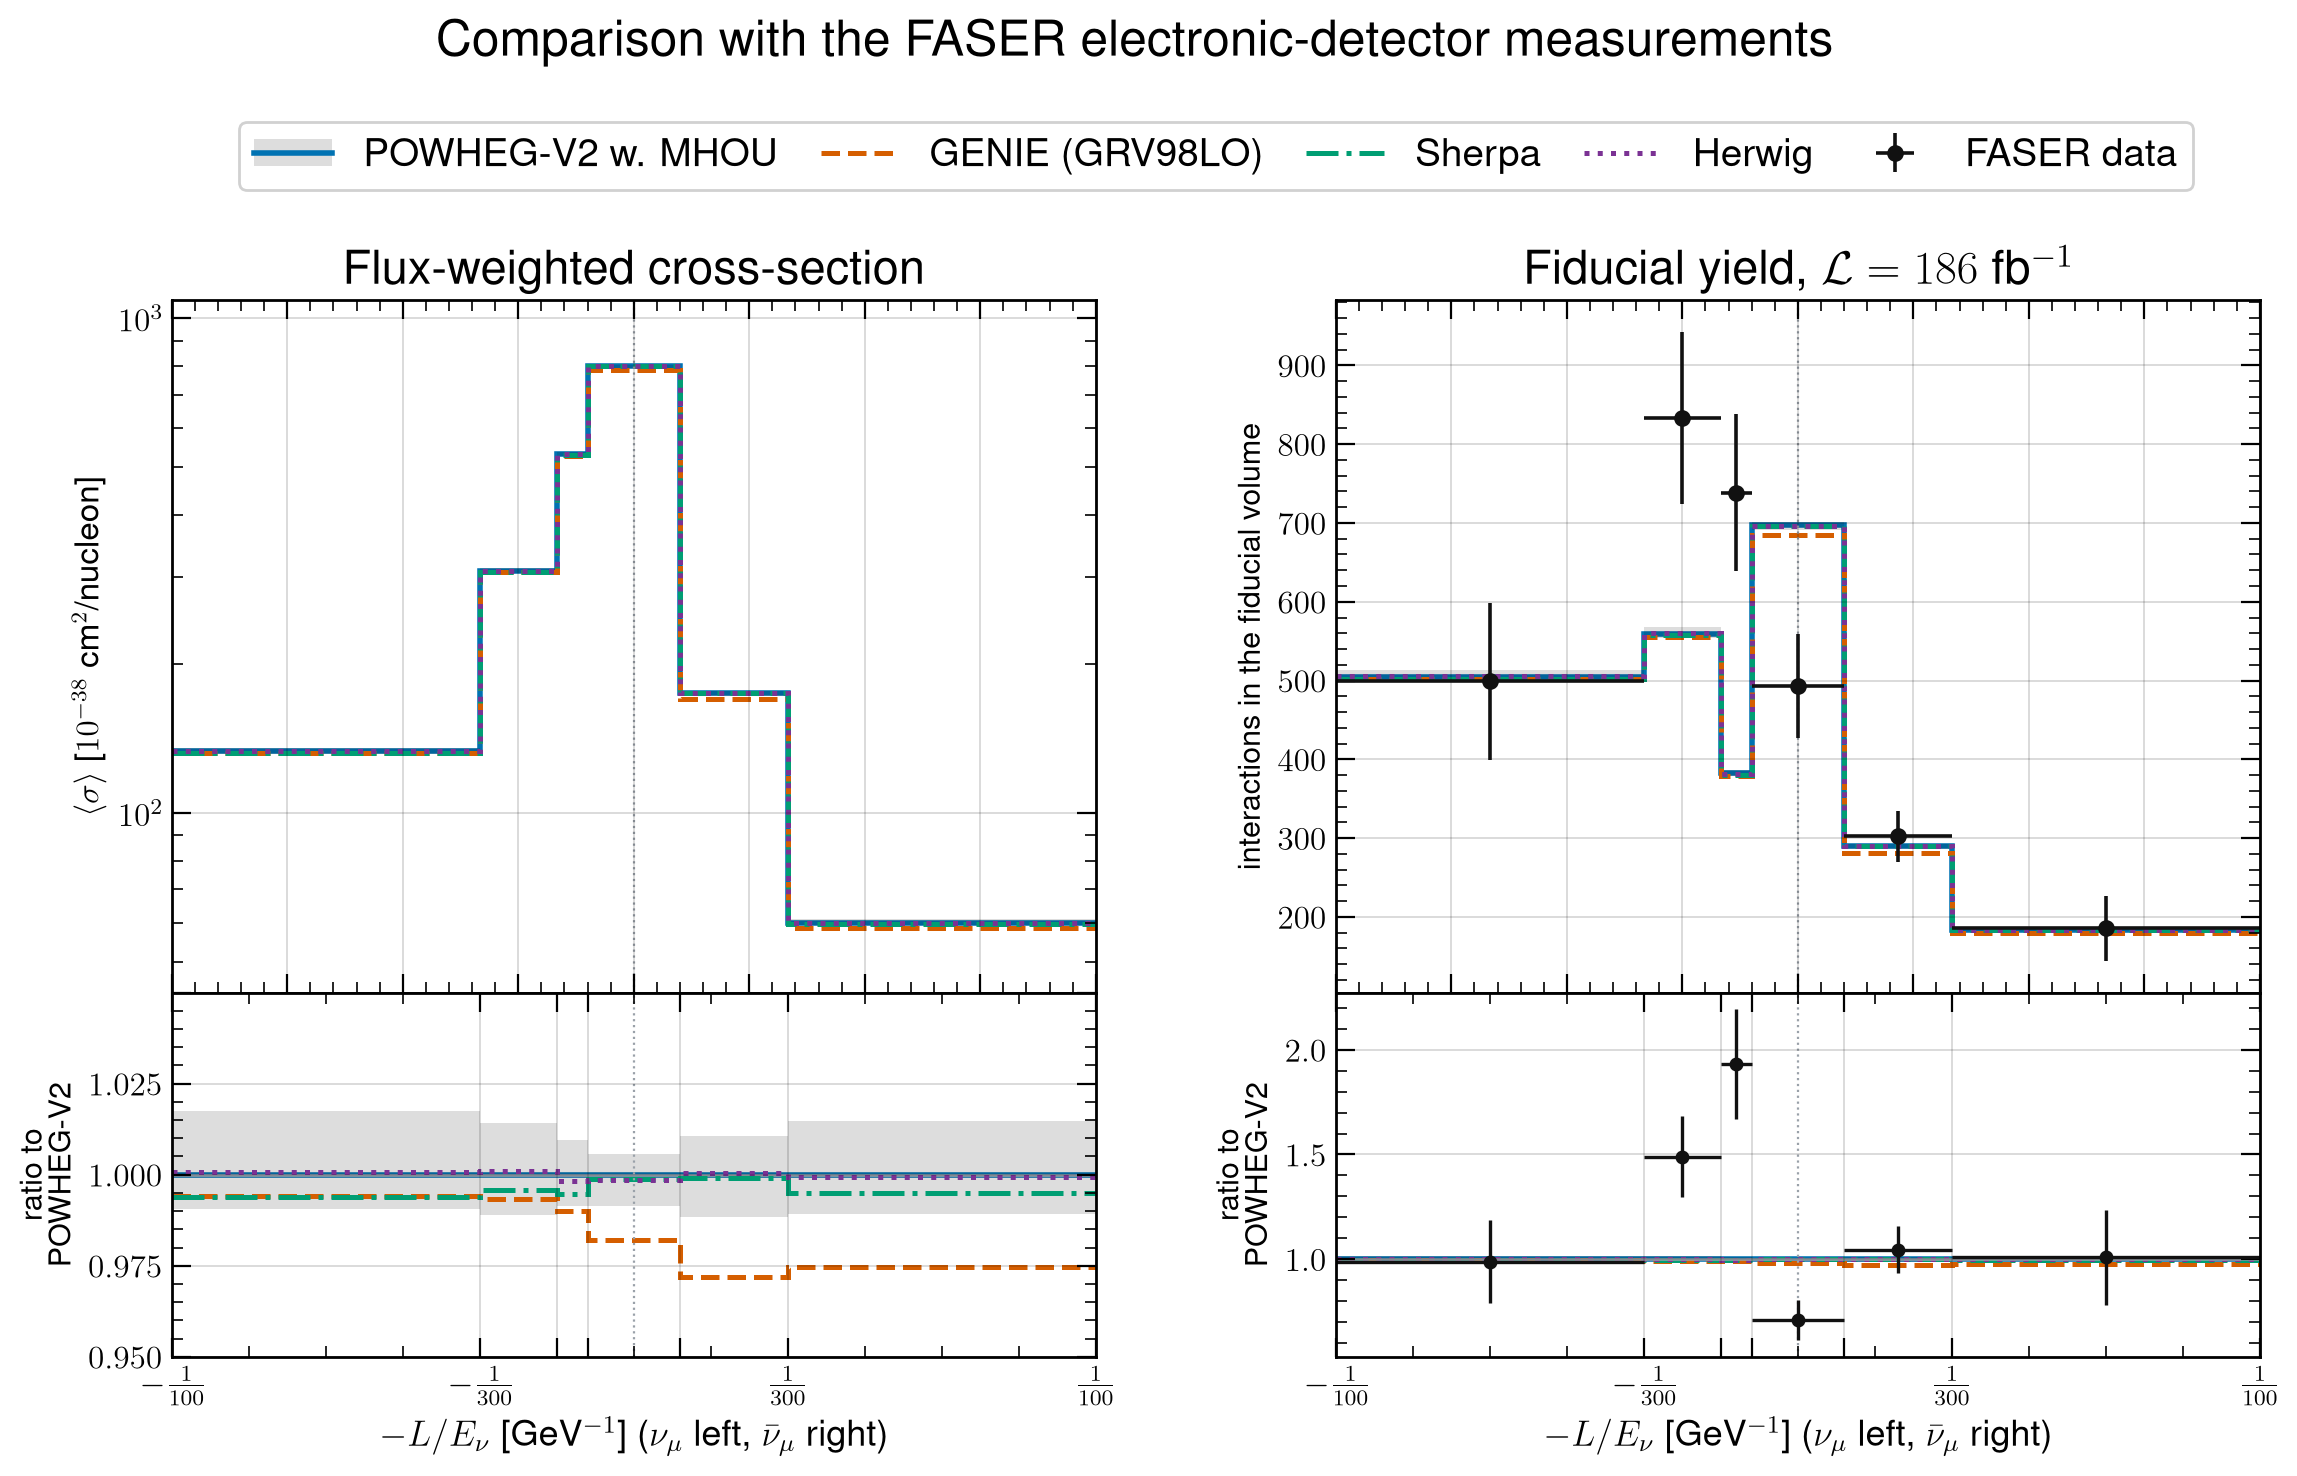
\includegraphics[width=0.99\textwidth]{figures/pp_faser_electronic.png}
  \caption{Left: predictions from \powhegtwo, \sherpa, \herwig, and \genie for the flux-weighted cross-section for CC DIS in the $-L/E_\nu$ kinematics of the FASER muon-neutrino electronic detector measurements of~\cite{FASER:2026enu2d}.
%
The central bin corresponds to the $\nu_{\mu}+\bar{\nu}_{\mu}$ sum, and the bottom panel displays the ratio to the \powhegtwo prediction.
%
The \powhegtwo, \sherpa, and \herwig predictions are complemented with the $Q^2< 4$~GeV$^2$ contribution taken from \genie to match the fiducial selection, see text.
%
  Right: the corresponding predictions for the number of muon-neutrino CC interactions expected for $\mathcal{L}=186$~fb$^{-1}$ compared to the unfolded FASER data~\cite{FASER:2026enu2d}. 
}
  \label{fig:faser-electronic}
\end{figure}
%%%%%%%%%%%%%%%%%%%%%%%%%%%%%%

From the comparisons of Fig.~\ref{fig:faser-electronic} one observes that the \sherpa and \herwig cross-sections agree with \powhegtwo to better than $1\%$ in every bin, and \genie to within $3\%$.
%
Without the extension below $Q^2=4$~GeV$^2$, \genie would instead lie up to $25\%$ above \powhegtwo in the two lowest $E_\nu$ bins, where this region is not negligible at the inclusive level. 
%
Concerning the comparison with the FASER measurements, the data agree with \powhegtwo within uncertainties in three of the six bins, but exceed it by $50\%$ and $90\%$ in the $300$--$1000$~GeV $\nu_\mu$ bins and fall $30\%$ below it above 1~TeV, differences which are much larger than the differences between theoretical predictions as well as the experimental uncertainties.
%
This discrepancy may indicate that the current predictions for the light-hadron fluxes that dominate muon-neutrino production need to be improved. 
%
In other words: for this specific observable, the data-vs-theory comparison is driven by the assumed neutrino fluxes and not by the modelling of the neutrino-nucleon scattering cross-section.

\paragraph{Charm production and the dimuon signal.}
\label{sec:faser-dimuon}

Charm production in neutrino DIS represents a powerful probe of the strangeness content of protons~\cite{Faura:2020oom,Gao:2017kkx} and nuclei.
%
Charm production can be measured at FASER through the emulsion detector, and a first search of this process was presented in~\cite{FASER:2026charm}.
%
Complementing these direct charm production measurements, FASER may be able to access this process by reconstructing the dimuon final state, Eq.~(\ref{eq:tierD}), via its tracking spectrometer.
%
In the dimuon process, the scattered muon is accompanied by an oppositely charged muon from the semileptonic decay of the charm hadron~\cite{Helenius:2024fow,Helenius:2025fpy,Helenius:2026uuz}.
%
While other neutrino experiments have measured the dimuon signal~\cite{NuTeV:2001dfo,NOMAD:2013hbk}, previous measurements involved much lower neutrino energies than those that FASER can reach.
%
Here we provide an initial estimate of the expected dimuon rates at the FASER electronic detector, and illustrate its PDF sensitivity by providing predictions for the dimuon yields for different PDF sets. 

Fig.~\ref{fig:dimuon-pdf} presents NLO predictions from \powhegtwo for the dimuon signal arising from charged-current DIS recorded in FASER's electronic detector assuming an integrated luminosity of $\mathcal{L}=300$~fb$^{-1}$, using the dimuon selection defined in Sect.~\ref{sec:faser-selections}.
  %
 Predictions are provided for different PDF sets at the following analysis levels: first, inclusive CC scattering within the fiducial volume, then, after requiring a charm tag (information only accessible at the truth level), then after requiring a semileptonic charm decay into a muon, and finally after requiring both muons inside the spectrometer acceptance and imposing three possible cuts on the total momentum of the subleading muon, $p_{\mu,\rm subl}$.   
 %
 Note that GRV98 does not provide a PDF uncertainty estimate.
%
The bottom panels display the ratio to NNPDF4.0 and also include the MHOUs which are always subdominant as compared to the differences between PDF sets. 

From Fig.~\ref{fig:dimuon-pdf} one observes that FASER, for the assumed integrated luminosity, should record between 10 and 30 dimuon events, depending on the choice of PDF set and on how strict the cut on $p_{\mu,\rm subl}$ is.
%
This cut is necessary to reduce the backgrounds, for example charged pions produced near the end of the tungsten target, which can traverse the spectrometer and mimic a muon, but with a softer momentum spectrum. 
%
Hence, given the predicted event yields, and provided systematic errors and background subtraction can be kept under control, it is possible that FASER reports an observation of the dimuon signal with the full Run 3 dataset.

Furthermore, Fig.~\ref{fig:dimuon-pdf} also displays a significant dependence on the choice of PDF: as compared to the reference NNPDF4.0, CT18 predicts around 20\% fewer events and GRV98 40\% fewer events.
%
In addition, the predictions from different PDF sets do not agree in all cases within their nominal uncertainties. 
%
Hence a measurement of the dimuon signal, already based on the Run 3 dataset, should provide information to constrain the strange PDFs of the nucleon complementing existing dimuon measurements at lower energies which are already part of global PDF fits. 
%
As mentioned above, additional constraints will be provided by FASER$\nu$ measurements~\cite{FASER:2026charm} of charm production (corresponding to the second column of Fig.~\ref{fig:dimuon-pdf}), where despite a lower efficiency for charm reconstruction of $\epsilon_c\sim 50\%$, the separation between signal and background events is greatly facilitated as compared to the dimuon final state. 

%%%%%%%%%%%%%%%%%%%%%%%%%%%%%%%%%%%%%%%%%%%%%%
\begin{figure}[!tbp]
  \centering
  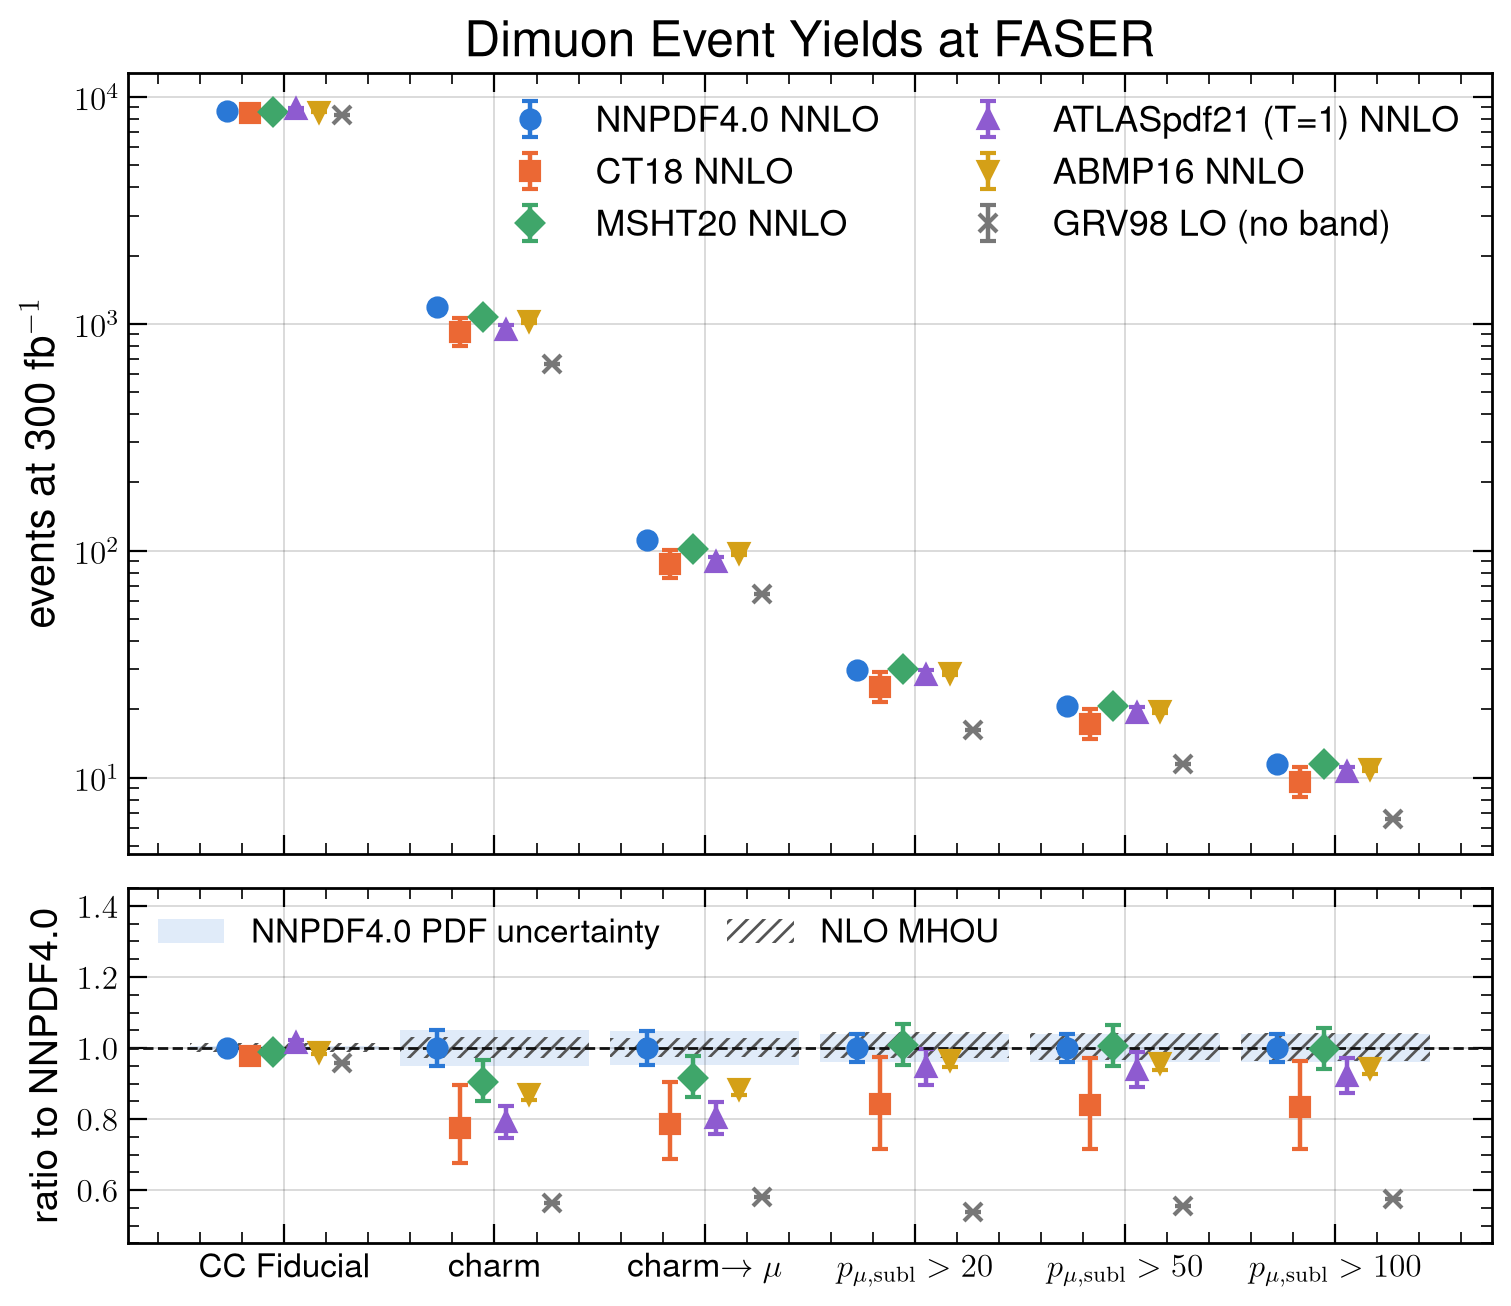
\includegraphics[width=0.80\textwidth]{figures/pp_faser_dimuon_pdf.png}
  \caption{
  NLO predictions from \powhegtwo for the dimuon signal ($\nu_\mu + \bar\nu_\mu$) arising from CC muon-neutrino DIS recorded in FASER's electronic detector for an integrated luminosity of $\mathcal{L}=300$~fb$^{-1}$. 
  %
 Predictions are provided for different PDF sets at the following analysis levels: inclusive CC scattering in the fiducial volume, after requiring a charm tag (information only accessible at the truth level), after requiring a semileptonic charm decay into a muon, and then requiring both muons inside the spectrometer acceptance and imposing three possible cuts on the total momentum of the subleading muon, $p_{\mu,\rm subl}$.   
 %
 GRV98 does not provide a PDF uncertainty estimate.
%
The bottom panels display the ratio to NNPDF4.0 and also include the MHOUs from \powhegtwo. }
  \label{fig:dimuon-pdf}
\end{figure}
%%%%%%%%%%%%%%%%%%%%%%%%%%%%%%%%%%%%%%%

\paragraph{Inclusive charged-hadron production in SIDIS.}
%
As a third representative application, we consider the possible measurement of the total charged-hadron production rate in semi-inclusive DIS.
%
Such a measurement would be enabled by the unique capabilities of FASER$\nu$, which reconstructs every charged track at the interaction vertex and hence can access single-inclusive hadron production, $\nu N \to \ell h X$, summing over all charged hadrons $h$ in the final state.
%
This is a process directly sensitive to the hadron fragmentation functions~\cite{Borsa:2021ran,Bertone:2017tyb,Bertone:2018ecm,Albino:2008gy}, and which can be evaluated up to NNLO in the QCD expansion both for charged-current~\cite{Bonino:2025ident,Bonino:2025qta} and for neutral-current scattering~\cite{Bonino:2024qbh,Goyal:2023zdi}, and for the polarised case in both currents~\cite{Goyal:2024tmo,Bonino:2024wgg,Bonino:2025sidis}.
%
In particular, this would be the first measurement of charged-hadron fragmentation in neutrino-initiated SIDIS at TeV energies.

To estimate the expected event yields, Fig.~\ref{fig:sidis-yields} displays predictions for the expected event yields in semi-inclusive charged-current DIS at FASER$\nu$ for $\mathcal{L}=300$ fb$^{-1}$ as a function of the SIDIS variable $z = E_{h^\pm}/\nu$, where $z$ corresponds to the fraction of the energy transfer carried by the reconstructed charged hadron $h^\pm$.
  %
  We evaluate total charged-hadron production summing over all stable charged hadrons (mostly pions and kaons, but also protons and hyperons) for events passing the FASER$\nu$ selection of Eq.~(\ref{eq:tierE}) and assuming an $80\%$ hadron selection efficiency, a conservative value given the single-film and tracking efficiencies of the FASER$\nu$ emulsion detector~\cite{FASER:2025qaf}, for $\nu_e+\bar{\nu}_e$  and $\nu_\mu+\bar{\nu}_\mu$ charged currents. 
%
The shaded band indicates the $z < 0.1$ region where fixed-order SIDIS calculations may not be reliable. 
%
While not shown here, charged-hadron production in muon DIS can also be evaluated using the same pipeline, and the event yields are substantially higher than those of the neutrino counterparts. 

%%%%%%%%%%%%%%%%%%%%%%%%%%%%%%%%%%%%%%%%%%%
\begin{figure}[!tbp]
  \centering
  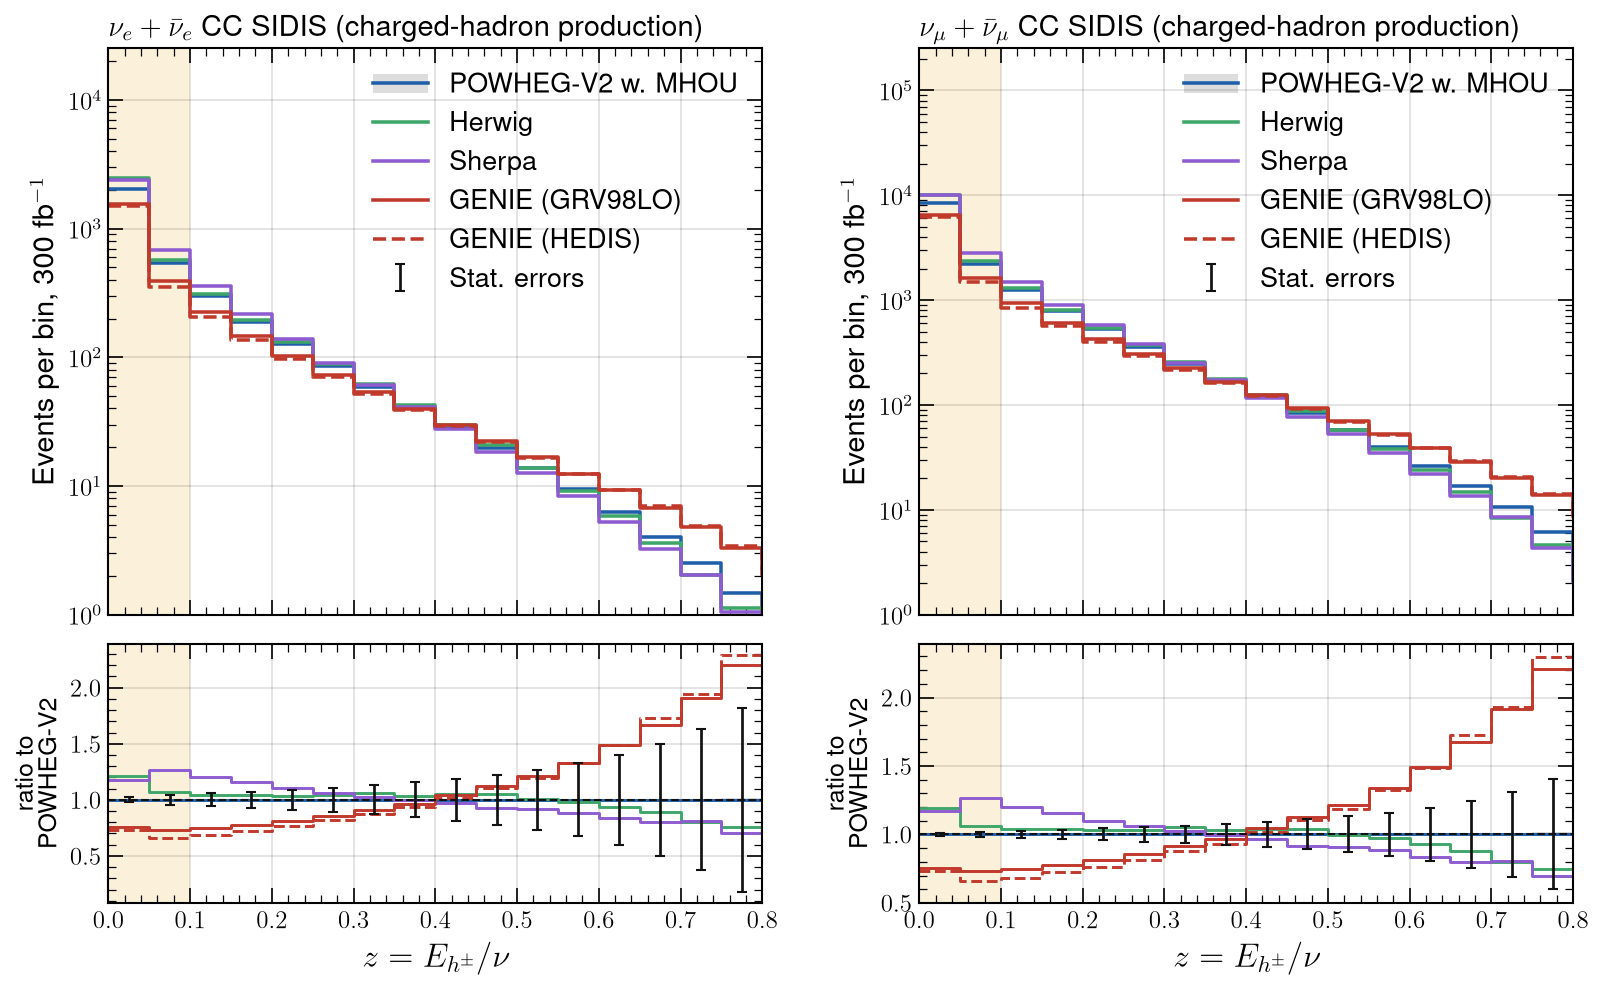
\includegraphics[width=0.98\textwidth]{figures/pp_sidis_yields.png}
  \caption{Predictions for the expected event yields in semi-inclusive charged-current DIS at FASER$\nu$ for $\mathcal{L}=300$ fb$^{-1}$ as a function of the SIDIS variable $z = E_{h^\pm}/\nu$.
  %
  We display the yields for SIDIS with charged-hadron production summing over all stable charged hadrons (mostly pions and kaons) and assuming an $80\%$ hadron selection efficiency, for $\nu_e+\bar{\nu}_e$ (left panel) and $\nu_\mu+\bar{\nu}_\mu$ (right panel) scattering. 
%
The shaded band indicates the $z < 0.1$ region where fixed-order SIDIS calculations may not be reliable. 
%
The bottom panels display the ratios to \powhegtwo, with error bars indicating the expected statistical uncertainty in each bin.
    }
  \label{fig:sidis-yields}
\end{figure}
%%%%%%%%%%%%%%%%%%%%%%%%%%%%%%%%%%%

From Fig.~\ref{fig:sidis-yields}, we expect that FASER$\nu$ should record around 900 (3700) charged hadrons in electron- (muon-)neutrino scattering, summing over neutrinos and antineutrinos, in the region $z>0.1$ where perturbative predictions are reliable.
%
Note that in Fig.~\ref{fig:sidis-yields} hadrons in a bin are not independent counts, since each event in general contains multiple charged hadrons within the FASER$\nu$ acceptance. 
%
Despite the steeply falling distribution in $z$, it is possible to cover up to $z\sim 0.4$--$0.5$ with sufficient statistics, especially in muon-neutrino SIDIS, hence accessing hadron fragmentation functions in kinematic regions which are currently poorly constrained. 
%
Concerning differences between generators,  \powhegtwo and \herwig agree at the few-per-cent level for most of the $z$ range (and never differ by more than 20\%), with \sherpa displaying somewhat larger differences both at small and large $z$.
%
Both \genie tunes predict a completely different hadron fragmentation distribution, underestimating the NLO rate by about 30\% at small $z$ and overestimating it by more than a factor of two at large $z$, highlighting that \genie, which fragments the hadronic system with the Lund string but without a preceding parton shower, predicts harder fragmentation than the three NLO-matched generators considered. 

The analysis of Fig.~\ref{fig:sidis-yields} strongly suggests that a first measurement of charged-hadron neutrino SIDIS at TeV energies should be possible with the full Run 3 dataset of FASER$\nu$, and the predicted statistical precision should be enough to distinguish between different calculations of hadron fragmentation, both those embedded in the hadronisation models used by the event generators as well as those based on fragmentation functions within the analytical QCD factorisation framework. 

We note again that in this study we do not account for (cold) nuclear final-state effects. 
%
The hard scattering process takes place inside a tungsten nucleus, which the outgoing quark must leave while undergoing parton shower and hadronisation. 
%
Interactions of both partons and hadrons with the cold nuclear medium will in general lead to the formation of more particles, thereby increasing the hadron multiplicity while decreasing the typical hadron energies and therefore the hadronic energy fraction $z$~\cite{Doradau:2024wli,deFlorian:2011fp}.
%
A complete theoretical model describing how parton showers evolve inside dense nuclei and how partons interact with cold nuclear matter is currently lacking. 
%
While these phenomena will be studied in detail at the Electron-Ion Collider (EIC)~\cite{Accardi:2012qut,AbdulKhalek:2021gbh}, the LHC neutrino and muon programme can perform the same measurements a decade in advance.